\documentclass[a4paper,12pt]{article}

\usepackage[utf8]{inputenc}
\usepackage[T1]{fontenc}
\usepackage[frenchb]{babel}
\usepackage{amsmath, amssymb}
\usepackage{graphicx}
\usepackage{hyperref}
\usepackage{float}
\usepackage[section]{placeins}
\usepackage[justification=centering]{caption}
\usepackage{subcaption}
\usepackage{wallpaper}
\usepackage{nomencl}
\usepackage{fancyhdr}
\usepackage{url}
\usepackage{siunitx}
\usepackage[left=3cm,right=3cm,top=3cm,bottom=5cm]{geometry}



% ---------- Page de garde -----------
\newcommand{\logoentreprise}[1]{\renewcommand{\logoentreprise}{#1}}
\newcommand{\nomentreprise}[1]{\renewcommand{\nomentreprise}{#1}}

\newcommand{\titre}[1]{\renewcommand{\titre}{#1}}
\newcommand{\intitule}[1]{\renewcommand{\intitule}{#1}}

\newcommand{\trigrammemention}[1]{\renewcommand{\trigrammemention}{#1}}
\newcommand{\master}[1]{\renewcommand{\master}{#1}}
\newcommand{\filiere}[1]{\renewcommand{\filiere}{#1}}

\newcommand{\eleve}[1]{\renewcommand{\eleve}{#1}}

\newcommand{\dates}[1]{\renewcommand{\dates}{#1}}

\newcommand{\promo}[1]{\renewcommand{\promo}{#1}}

\newcommand{\annee}[1]{\renewcommand{\annee}{#1}}

\newcommand{\tuteurecole}[1]{\renewcommand{\tuteurecole}{#1}}
\newcommand{\tuteurentreprise}[1]{\renewcommand{\tuteurentreprise}{#1}}

% Formatte les pages (header, marges, image, ...)
\newcommand{\fairemarges}{
    \makenomenclature{}
    \pagestyle{fancy}
    \fancyheadoffset{1cm}
    \setlength{\headheight}{2cm}
    \lhead{
\includegraphics[scale=0.5]{figures/tps.png}}
    \rhead{\nouppercase{\leftmark}}
    \rfoot{\thepage}
    \cfoot{}
    \lfoot{\trigrammemention}
}

% Créer la page de garde
\newcommand{\fairepagedegarde}{
    \begin{titlepage}

        \centering{} %Centraliser le contenu

        % Logo Entreprise x ecole
        \begin{figure}
            \begin{subfigure}{.5\textwidth}
                \centering{}
                
\includegraphics[width=0.6\textwidth]{figures/tps.png}\par\vspace{1cm}
            \end{subfigure}%
            \begin{subfigure}{.5\textwidth}
                \centering{}
                
\includegraphics[width=0.6\textwidth]{figures/imt.png}\par\vspace{1cm} %%
            \end{subfigure}
        \end{figure}

        \vspace{0.5cm}
        {\scshape{} \intitule{} \par}
        \vspace{0.5cm}

        % Titre du rapport
        \rule{\linewidth}{0.2 mm} \\[0.4 cm]
        {\Large\bfseries{} \titre{} \par} \
        \rule{\linewidth}{0.2 mm} \\[1.0 cm]

        % Nom de l'étudiant
        {\eleve{} \par}
        \vspace{1.0cm}

        % Promotion
        {\scshape{} Promotion \promo{} \par}
        \vspace{1.0cm}

        % Parcours de l'étudiant
        {\scshape{} \filiere{} \\ \master{} \par}
        \vspace{1cm}

        % Année universitaire
        {\large{} \annee{} \par}
        \vspace{1cm}

        % Dates
        {\large{} \dates{} \par}
        \vspace{1.5cm}

        % Bas de page
        \begin{minipage}{0.4\textwidth}
            \begin{flushleft}
                \emph{\textbf{Organisme d'accueil}}\\
                \text{\nomentreprise}\\
                \includegraphics[width=0.4\textwidth]{\logoentreprise} \\
            \end{flushleft}
        \end{minipage}
        ~
        \begin{minipage}{0.4\textwidth}
            \begin{flushright}
                \emph{\textbf{Tuteur école:}} \\
                \tuteurecole{} \\
            \end{flushright}
            \begin{flushright}
                \emph{\textbf{Tuteur entreprise:}} \\
                \tuteurentreprise{} \\
            \end{flushright}
        \end{minipage}\\[2cm]

        \vfill{}


    \end{titlepage}
    \newpage{}
}


%---------- Métadonnées du document ----------
\title{Rapport de stage}
\author{Romain BOURDAIN}
\date{\today}


%----------- Charge la biblio ---------
\addbibresource{bibliography.bib} %Import the bibliography file

% ---------- Document ----------
\begin{document}

\pagenumbering{roman} % On numérote le début du rapport en nombres Romains (pas moi haha)

% ---------- Informations du rapport ----------
\logoentreprise{figures/cover/entreprise.png}
\nomentreprise{Icube}

% Titre du rapport
\titre{Création d'un langage de programmation pédagogique pour la vérification de programmes concurrents}
\intitule{Mémoire de stage de 2ème année}

% Pour le bas de la page
\trigrammemention{TPS}

% Nom de la filière
\filiere{Filière Informatique et réseau}
\master{Science des données et systèmes complexes}

% Votre nom
\eleve{BOURDAIN Romain}

% La promo
\promo{2025}

% L'année universitaire en cours
\annee{2023/2024}

% Les dates du stage
\dates{03/06/2024 - 23/08/2024}


% Le nom et adresse du tuteur école
\tuteurecole{
    \textsc{HABET Adlane} \\
    habed@unistra.fr
}

% Le nom et adresse du tuteur entreprise
\tuteurentreprise{
    \textsc{BRAMAS Quentin} \\
    bramas@unistra.fr
}


%----------- Initialisation -------------------
\fairemarges{} % Afficher les marges
\fairepagedegarde{} % Afficher la page de garde
\setcounter{figure}{0}



%----------- Remerciements -------------------
\section*{Remerciements}
\addcontentsline{toc}{section}{Remerciements}
\lipsum[2]
\newpage{}

%------------ Table des matières ----------------
\tabledematieres{}

%------------ Corps du rapport ----------------
\pagenumbering{arabic} % On numerote maintenant en chiffres arabes

%------------ Introduction ----------------
\section*{Introduction}
\addcontentsline{toc}{section}{Introduction}
\lipsum[2]

% Tu pourrais ajouter une section sur la problématique du stage avant d'entrer dans le contexte, pour expliquer en quoi consiste le problème que ton travail cherche à résoudre et pourquoi il est important.

\newpage{}

\section{Présentation du laboratoire}
\subsection{Présentation d'Icube}

Icube est un laboratoire de recherche fondé en 2013 avec le soutien de l'université de Strasbourg, le CNRS, l'ENGEES et l'INSA de Strasbourg. Spécialisé dans les sciences de l'ingénieur, de l'informatique et de l'imagerie, Icube représente l'une des communauté de recherche les plus importantes avec plus de 650 membres en 2018. Les domaines de recherche du laboratoire regroupent la mécanique, la photonique, l'électronique, l'informatique, le traitement de l'image, l'automatique et la robotique, un large éventail de domaines permettant de façonner l'avenir et la société.

La recherche est organisée en 4 départements couvrant les disciplines fondamentales du laboratoire :
\begin{enumerate}
    \item{} Le département Informatique Recherche ;
    \item{} Le département Imagerie, Robotique, Télédétection et Santé ;
    \item{} Le département Électronique du Solide, Systèmes et Photonique ;
    \item{} Le département Mécanique.
\end{enumerate}

\begin{figure}[H]
    \centering
    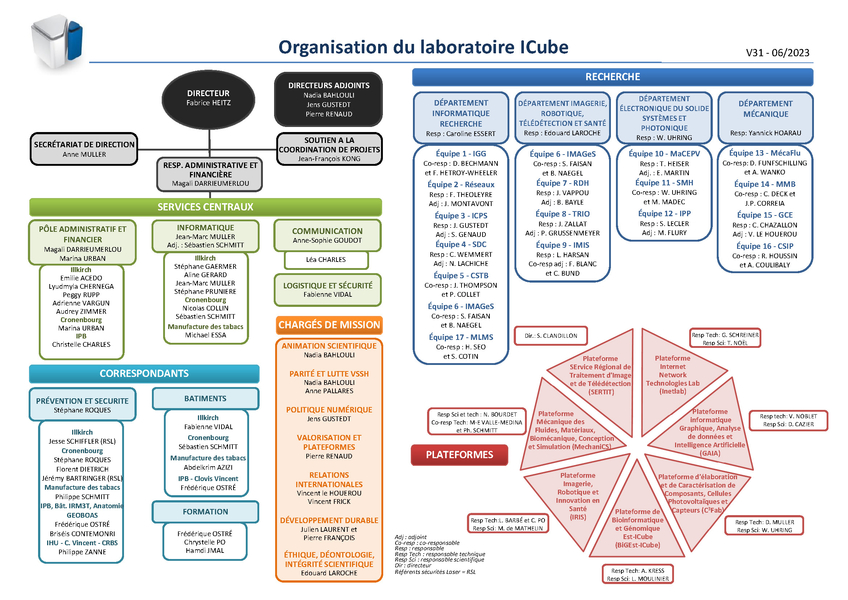
\includegraphics[scale=0.3]{figures/presentation/organigramme.jpg}
    \caption{Organigramme d'ICube}
    \label{fig1}
\end{figure}

\subsection{L'équipe reseau}

L'équipe réseau dans laquelle le stage s'est déroulé fait partie du département informatique et recherche. Cette équipe conceptualise des algorithmes et des protocoles d'architecture de communication. Ses domaines d'étude sont les réseaux de bordure, ls réseaux de cœur ainsi que les algorithmes distribués.

Cette équipe est composée de 11 membres permanents, 2 membres associés, 2 post-doctorants et 5 doctorants. Les membres permanents sont pour la plupart des enseignants-chercheurs de l'université de Strasbourg.
\newpage{}

\section{Contexte du stage}

Ce chapitre présente un état de l'art concernant la création d'un langage de programmation dans le domaine de la vérification de programmes concurrents.

\subsection{Les objectifs du langage Althread}
\subsubsection{Validation de modèles distribués}
L'objectif principal de ce langage est de modéliser et de valider des modèles d'algorithmes distribués. Son usage est à but purement pédagogique pour les étudiants de l'université de Strasbourg.
\subsubsection{Facilité d'apprentissage}
\subsubsection{Accessibilité du langage}
\subsubsection{Licence et OpenSource}
\subsection{Langages similaires}
\subsubsection{Le langage Promela}
\subsubsection{Le Langage TLA+}
\subsection{État du projet avant le stage}
\newpage{}

\section{Analyses lexicale et syntaxique}
\subsection{Principe de l'analyse lexicale}
Dans la conception d'un langage de programmation, l'analyse lexicale est une étape inévitable. L'objectif est de transformer une suite de mots, à savoir le code source, en une suite de \textit{tokens} qui seront plus facilement interprétables par une machine. Un \textit{token} un couple composé d'un nom et d'une valeur optionnelle. Par exemple, dans le langage C, les mots clé \textit{if}, \textit{while}, \textit{return}, les ponctuation, les noms de variable ou même les littéraux \textit{true}, \textit{8.23} ,\textit{"Hello World"} sont des tokens.

\begin{figure}[H]
    \centering
    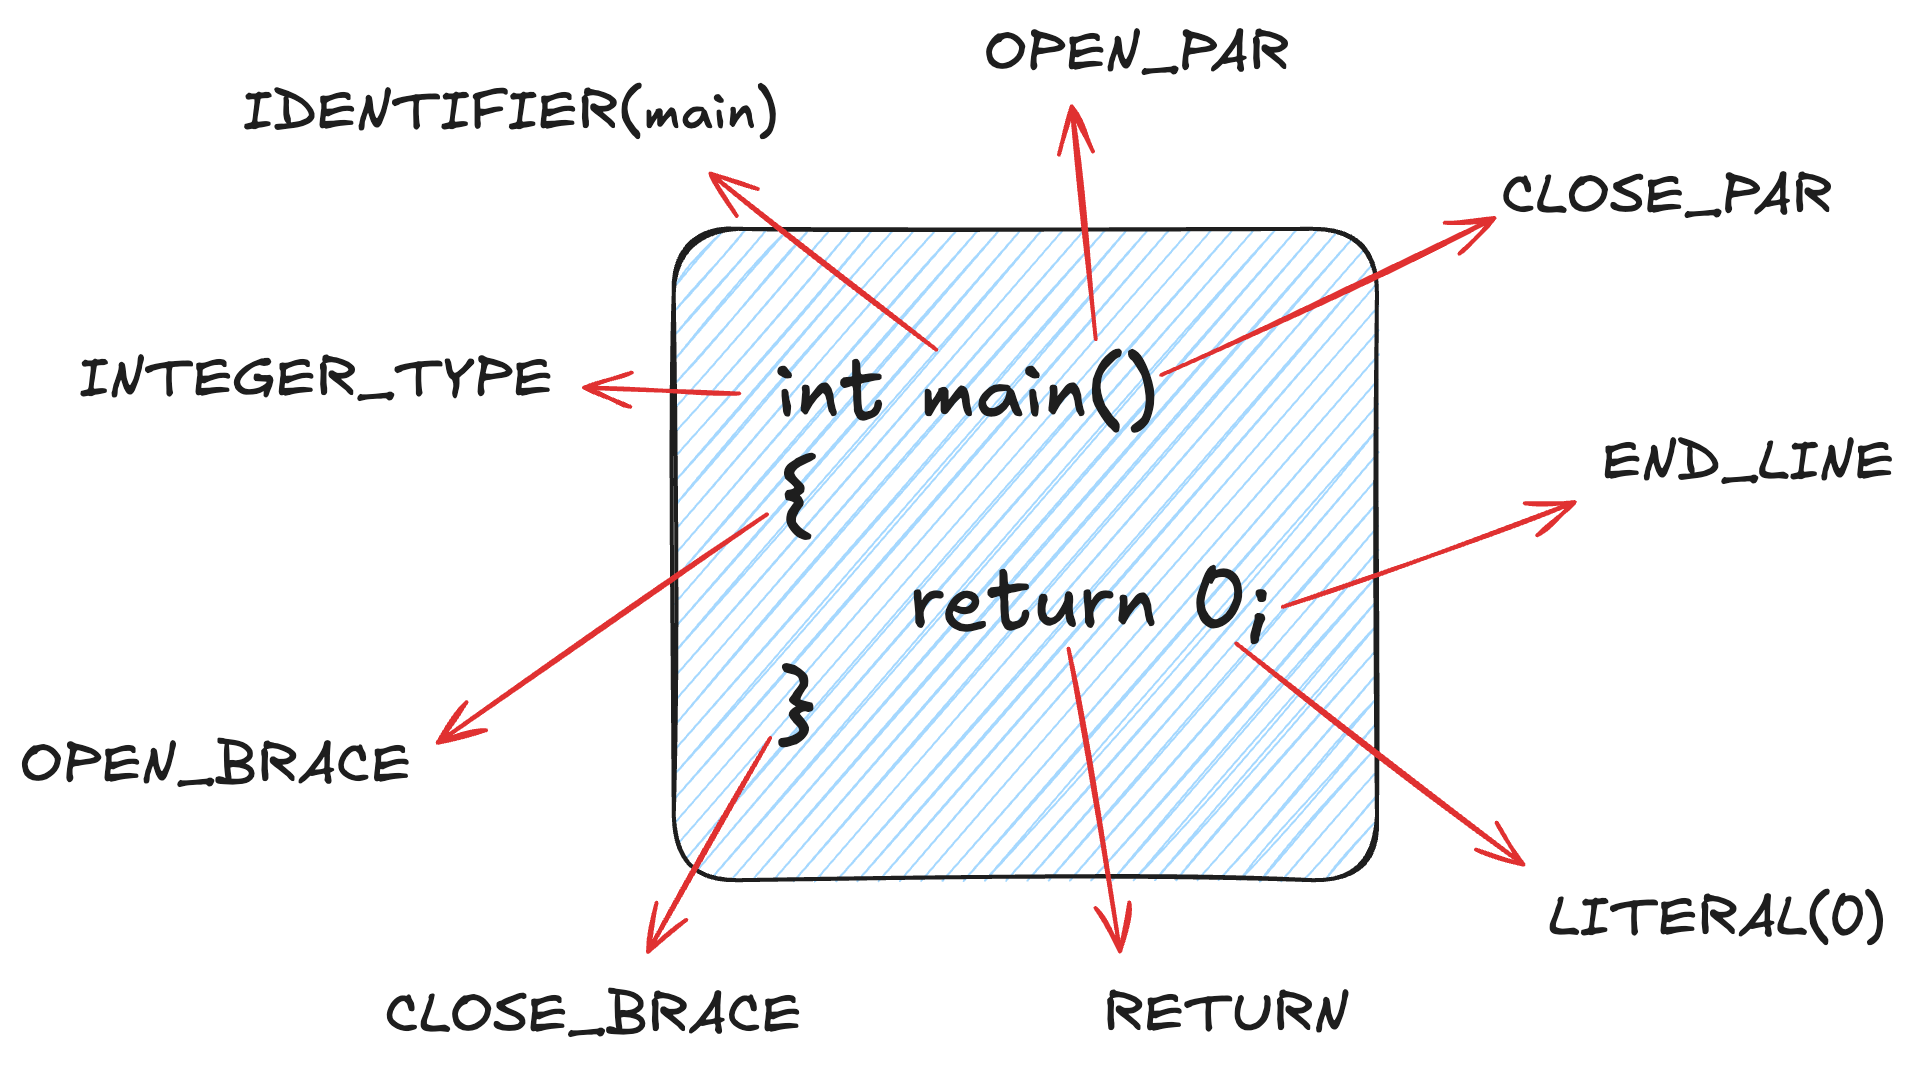
\includegraphics[width=12cm]{figures/syntaxe/lexing.png}
    \caption{Analyse lexicale d'un code en C}
    \label{fig2}
\end{figure}

C'est également à cette étape que certaines premières erreurs sont détectées, comme les erreurs de syntaxe. Par exemple, un mot clé ou un symbole non prévu par le langage va générer une erreur de syntaxe.

Certains tokens doivent cependant avoir une valeur associée pour être interprétables. Par exemple, un nombre entier doit être associé à une valeur numérique pour être utilisé dans un programme.

L'avantage des tokens par rapport au texte brut est que les tokens sont beaucoup plus facile à manipuler. Un exemple simple pour comprendre l'avantage des tokens est l'utilisation du signe \textquote{=} en C. Ce signe est utilisé pour l'affectation de variables, mais aussi pour la comparaison de deux valeurs. L'analyse lexicale permet de distinguer ces deux utilisations du signe \textquote{=}.

\subsection{Syntaxe d'Althread}
Dans le but d'obtenir un langage facile à prendre en main, la syntaxe d'Althread est proche de celle des langages existants comme le C, le rust et même promela dans certains cas. Cette section détaille les choix faits concernant la syntaxe du langage.

\subsubsection{Syntaxe pour les instructions}
Comme en langage C, les instructions en Althread sont séparées par un point-virgule.
\subsubsection{Structure du programme en blocks}
\subsubsection{Grammaire}

La grammaire d'un langage de programmation est la définition formelle du langage. Elle permet de définir les règles de syntaxe du langage et de déterminer si un programme est syntaxiquement correct.
\newpage{}

\section{Production de code intermédiaire}
Après l'analyse lexicale et syntaxique vient l'étape de production de code intermédiaire. L'objectif de cette étape est de

\subsection{Génération de l'AST}
\subsection{Structure de Node}
\subsection{Typage des données}
\newpage{}

\section{Interprétation}
\subsection{Langage interprété vs langage compilé}
\subsection{Gestion de l'arithmétique}
\subsection{Table des symboles}
\subsection{Gestion des processus}
\subsection{Gestion des tests}

\newpage{}

\section{Outils pour le développement}
\subsection{Deboggueur}
\subsection{Documentation d'Althread}
\subsubsection{Utilisation de Docusaurus}
\subsubsection{Structure de la documentation}
\newpage{}

\section{Tests du code source}
\subsection{Mise en place de tests unitaires}
\subsection{Traduction de programmes Promela en Althread}
\newpage{}

\section{Améliorations futures}
\subsection{Amélioration de l'environnement d'exécution}
\subsection{Implémentation des channels}
\subsection{Mise en place d'outils pour le développement}
\newpage{}

%------------ Conclusion personnelle ----------------
\section*{Conclusion personnelle}
\addcontentsline{toc}{section}{Conclusion personnelle}
\lipsum[2]
\newpage{}

%------------ Conclusion ----------------
\section*{Conclusion}
\addcontentsline{toc}{section}{Conclusion}
\lipsum[2]
\newpage{}

%------------ Bibliographie ----------------
\section*{Bibliographie}
\addcontentsline{toc}{section}{Bibliographie}
Let's cite! Einstein's journal paper \cite{einstein} and Dirac's
book \cite{dirac} are physics\-related items.

\printbibliography{}
\newpage{}

%------------ Annexe ----------------
\section*{Annexe}
\addcontentsline{toc}{section}{Annexe}
\lipsum[2]
\newpage{}

%----------- Abstract -------------------
\vspace*{\stretch{1}}

\begin{center}
    \bf{} Resumé
\end{center}
\lipsum[1]

\vspace*{\stretch{1}}

\begin{center}
    \bf{} Abstract
\end{center}
\lipsum[1]

\vspace*{\stretch{1}}
\newpage{}


\end{document}